\chapter{เอกสารและงานวิจัยที่เกี่ยวข้อง}

\paragraph{}
บทนี้เป็นการทบทวนวรรณกรรม เอกสาร และงานวิจัยที่เกี่ยวข้องกับแนวคิดหลักและวิธีการที่ใช้ในการวิจัยนี้ โดยมีจุดมุ่งหมายเพื่อสร้างฐานความรู้ที่แข็งแกร่งและระบุช่องว่างทางการวิจัยที่โครงการนี้มุ่งเน้นแก้ไข เนื้อหาจะแบ่งออกเป็นแนวคิดพื้นฐานเกี่ยวกับระบบขับขี่อัตโนมัติ การสร้าง Scenario โครงสร้างข้อมูล Knowledge Graph และการใช้ LLM ในการประมวลผลภาษาธรรมชาติ

\section{แนวคิดพื้นฐานและทฤษฎีที่เกี่ยวข้อง}

\subsection{Ego Vehicle}
\paragraph{}
ในบริบทของการจำลองสถานการณ์และการทดสอบระบบขับขี่อัตโนมัติ คำว่า Ego vehicle หมายถึง ยานพาหนะหลักที่กำลังถูกทดสอบหรือประเมินผล Ego Vehicle คือรถยนต์ที่ติดตั้งระบบขับขี่อัตโนมัติ (ADS) ซึ่งเป็นหัวใจสำคัญของการทดลอง โดยมุมมอง, การรับรู้, การตัดสินใจ, และการกระทำทั้งหมดของรถคันนี้จะถูกบันทึกและวิเคราะห์เพื่อประเมินประสิทธิภาพและความปลอดภัยของระบบ

\subsection{Operational Design Domain}\label{sec:ODD}
\paragraph{}
Operational Design Domain (ODD) คือชุดของเงื่อนไขการปฏิบัติงานที่กำหนดไว้ล่วงหน้า เช่น สภาพภูมิอากาศ สภาพถนน ความเร็วสูงสุด ซึ่งระบบขับขี่อัตโนมัติ (ADS) ได้รับการออกแบบมาให้ทำงานได้อย่างปลอดภัย ODD เป็นแนวคิดที่สำคัญอย่างยิ่งในการประเมินความปลอดภัย เนื่องจากช่วยกำหนดขอบเขตการทดสอบให้ชัดเจน งานวิจัยนี้ได้ใช้ ODD ที่กำหนดโดย Japan Automobile Manufacturers Association (JAMA)เป็นข้อจำกัดหลักในการกรองและสร้าง Scenario เพื่อให้ชุดทดสอบมีความสอดคล้องกับขีดความสามารถของระบบที่กำลังประเมิน

\subsection{Knowledge Graph}\label{sec:KG}
\paragraph{}
Knowledge Graph เป็นรูปแบบการนำเสนอข้อมูลเชิงความหมาย (Semantic Data Structure) ที่ใช้โหนด (Nodes) และขอบ (Edges/Relationships) เพื่อแสดงถึงเอนทิตี (Entities) และความสัมพันธ์ระหว่างเอนทิตีเหล่านั้น บทบาทของ KG ในงานวิจัยนี้คือการทำหน้าที่เป็น Semantic Backbone สำหรับข้อมูลอุบัติเหตุ ทำให้สามารถจัดเก็บข้อมูลที่สกัดจากรายงานอุบัติเหตุในรูปแบบที่มีโครงสร้างและอนุมาน (Inference) ข้อมูลที่ขาดหายไปได้ นอกจากนี้ยังช่วยรักษาความต่อเนื่องเชิงเหตุผล (Causal Continuity) ของเหตุการณ์ที่เกิดขึ้นในอุบัติเหตุ

\subsection{การประมวลผลภาษาธรรมชาติ}\label{sec:NLP}
\paragraph{}
การประมวลผลภาษาธรรมชาติ หรือ Natural Language Processing (NLP) เป็นสาขาย่อยหนึ่งของปัญญาประดิษฐ์ (AI) และวิทยาการคอมพิวเตอร์ ที่มุ่งเน้นการสร้างปฏิสัมพันธ์ระหว่างคอมพิวเตอร์กับภาษามนุษย์ เป้าหมายหลักของ NLP คือการทำให้คอมพิวเตอร์สามารถ "เข้าใจ" ตีความ และสร้างภาษาของมนุษย์ได้ในลักษณะที่มีประโยชน์ ซึ่งครอบคลุมงานหลากหลายประเภท เช่น การสกัดข้อมูล (Information Extraction) การแปลภาษาด้วยเครื่อง (Machine Translation) และการวิเคราะห์ความรู้สึก (Sentiment Analysis) ในงานวิจัยนี้ เทคนิค NLP เป็นหัวใจสำคัญในการแปลงรายงานอุบัติเหตุที่อยู่ในรูปแบบข้อความที่ไม่มีโครงสร้าง ให้กลายเป็นข้อมูลเชิงลึกที่มีความหมายและนำไปใช้ต่อได้

\subsection{Large Language Model}
\paragraph{}
Large Language Model (LLM) เป็นโมเดลปัญญาประดิษฐ์ที่ได้รับการฝึกฝนด้วยข้อมูลจำนวนมหาศาล เพื่อทำความเข้าใจและสร้างภาษาธรรมชาติ LLM มีความสามารถในการสกัดข้อมูลที่ซับซ้อนจากข้อความที่ไม่มีโครงสร้าง (Unstructured Text) งานวิจัยนี้ใช้ LLM ในการสกัดข้อมูลอุบัติเหตุจากรายงานที่เป็นข้อความ โดยมีการนำเทคนิค Schema-guided LLM มาใช้เพื่อเพิ่มความน่าเชื่อถือและความสม่ำเสมอของข้อมูลที่สกัดได้

\subsection{Schema-guided Large Language Model}\label{sec:sgLLM}
\paragraph{}
LLM เป็นเครื่องมือที่มีประสิทธิภาพในการประมวลผลภาษาธรรมชาติ (NLP) \cite{khot2024prompting} งานวิจัยนี้ใช้เทคนิค Schema-guided LLM เพื่อควบคุมและกำหนดทิศทางการสกัดข้อมูลจากรายงานอุบัติเหตุที่เป็นข้อความ (Unstructured Text) ให้เป็นข้อมูลที่มีโครงสร้าง (Structured Data) ตาม Schema ที่ออกแบบไว้ล่วงหน้า \cite{liyan2022analysis} การควบคุมด้วย Schema นี้ช่วยเพิ่มความน่าเชื่อถือและความสม่ำเสมอของข้อมูลที่สกัดได้ ก่อนนำไปสร้างเป็น Knowledge Graph \cite{liyan2022analysis}

Schema-guided LLM ถูกใช้เพื่อแก้ไขปัญหาความไม่สมบูรณ์และความกำกวมของข้อมูลในรายงานอุบัติเหตุจริง (เช่น CIREN หรือ GIDAS) \cite{nhtsa_ciren, gidas_study} ซึ่งรายงานเหล่านี้มักถูกบันทึกในรูปแบบข้อความอิสระ (Free Text) ที่ขาดมาตรฐาน การใช้ Schema เป็น Blueprint หรือ Ontology ที่กำหนดไว้ล่วงหน้าจะทำหน้าที่เป็น "สัญญา" ในการสกัดเอนทิตี, คุณลักษณะ, และความสัมพันธ์ที่จำเป็นให้ครบถ้วน

เพื่อเพิ่มความเข้าใจในกระบวนการสกัดข้อมูลโดย Schema-guided LLM ขอนำเสนอตัวอย่างการแปลงรายงานอุบัติเหตุที่ไม่มีโครงสร้าง (Narrative) ให้อยู่ในรูปแบบข้อมูลที่มีโครงสร้าง (Extracted Feature) ซึ่งเป็นขั้นตอนสำคัญก่อนการสร้าง Knowledge Graph \cite{bagschik2018ontology}:

\begin{table}[htbp]
\centering
\caption{ตัวอย่างการสกัดข้อมูลโดย Schema-guided LLM: รายงานอุบัติเหตุ C00013}
\label{tab:sgllm_example}
\begin{tabularx}{\textwidth}{|p{0.48\textwidth}|X|}
\hline
\rowcolor{gray!20} รายงานอุบัติเหตุ (Unstructured Text: Case C00013) & ข้อมูลที่มีโครงสร้าง (Structured Data/Extracted Feature) \\
\hline
A two-vehicle collision occurred at a signalized urban intersection during daylight hours. Vehicle 1, a red fire truck traveling eastbound, entered on a green signal but came to a complete stop in the middle of the intersection. Vehicle 2, a white Honda compact SUV traveling southbound, entered against a red signal and struck the right passenger side of Vehicle 1. & \textbf{1. World/Environment:} \newline
\quad $\bullet$ Road Type: Urban intersection \newline
\quad $\bullet$ Signal Status: Functioning properly \newline
\quad $\bullet$ Time of Day: Daylight hours \newline
\quad $\bullet$ Road Condition: Dry \newline
\textbf{2. Actors:} \newline
\quad $\bullet$ Vehicle 1 (Target): Fire truck, traveling eastbound \newline
\quad $\bullet$ Vehicle 2 (Ego/ADS Candidate): White Honda compact SUV, traveling southbound \newline
\textbf{3. Scenario Sequence (Events):} \newline
\quad $\bullet$ Event 1 (V1): Stop in intersection (despite green light) \newline
\quad $\bullet$ Event 2 (V2): Encroachment (entered against red light) \newline
\quad $\bullet$ Event 3: Collision (V2 struck V1's right passenger side) \newline
\textbf{4. Outcome Metrics:} \newline
\quad $\bullet$ Injury Severity (V1 Driver): Moderate \newline
\quad $\bullet$ Injury Severity (V2 Driver): Minor \\
\hline
\end{tabularx}
\end{table}

\paragraph{}
ข้อมูลที่มีโครงสร้างดังกล่าว (ซึ่งอาจถูกเรียกว่า Extracted Feature หรือ JSON/XML output) เป็นรากฐานสำคัญที่ช่วยให้การแปลงเป็น Knowledge Graph ในขั้นตอนถัดไปเป็นไปได้อย่างแม่นยำและสม่ำเสมอ นอกจากนี้ การใช้ Schema ยังช่วยลดปัญหาความผิดพลาดในการอนุมานของ LLM (Hallucination) โดยเฉพาะในการสกัดความสัมพันธ์เชิงเหตุผลที่ซับซ้อน

\subsection{กรณีขอบเขต (Edge Case)}
\paragraph{}
หนึ่งในความท้าทายที่สำคัญที่สุดในการทดสอบระบบขับขี่อัตโนมัติ (ADS) คือการค้นหาสถานการณ์ที่เรียกว่า กรณีขอบเขต (Edge Case) ซึ่งหมายถึงสถานการณ์ที่เกิดขึ้นไม่บ่อยนัก มีความซับซ้อน หรืออยู่ ณ ขีดจำกัดของความสามารถที่ระบบได้รับการออกแบบมาให้รับมือ \cite{koopman2017autonomous} สถานการณ์เหล่านี้คือจุดที่ระบบมีโอกาสล้มเหลวหรือทำงานผิดพลาดได้มากที่สุด ตัวอย่างที่เข้าใจง่ายคือ "คนเดินถนนที่ปรากฏตัวจากมุมอับสายตาหลังรถบัสที่จอดอยู่" ซึ่งเป็นเหตุการณ์ที่คาดเดาได้ยากและต้องการการตอบสนองที่รวดเร็วจากระบบ

\paragraph{}
อย่างไรก็ตาม Edge Case ที่เกิดขึ้นในโลกแห่งความเป็นจริงมักมีความซับซ้อนกว่านั้นมาก โดยอาจประกอบด้วยลำดับเหตุการณ์ที่ต่อเนื่องกัน การตัดสินใจที่ผิดพลาดของผู้ขับขี่หลายคน หรือปัจจัยแวดล้อมที่ไม่ปกติ ดังแสดงในรูปที่~\ref{fig:edge_case_example} ซึ่งเป็นตัวอย่างสถานการณ์ที่สกัดมาจากรายงานอุบัติเหตุจริง สถานการณ์นี้ถือเป็น Edge Case ที่ดีเยี่ยมสำหรับการทดสอบ เนื่องจากเกี่ยวข้องกับการที่ยานพาหนะคันหนึ่งขับข้ามเส้นทึบเข้ามาในเลนสวนทาง ทำให้ผู้ขับขี่ทั้งสองฝ่ายต้องตัดสินใจหักหลบพร้อมกันในเวลาอันสั้น และจบลงด้วยการชนประสานงา ซึ่งเป็นสถานการณ์ที่ทดสอบความสามารถของ ADS ในการประเมินความเสี่ยงและเลือกการกระทำที่ลดความรุนแรงของอุบัติเหตุ (Damage Mitigation) ได้เป็นอย่างดี

\begin{figure}[htbp]
    \centering
    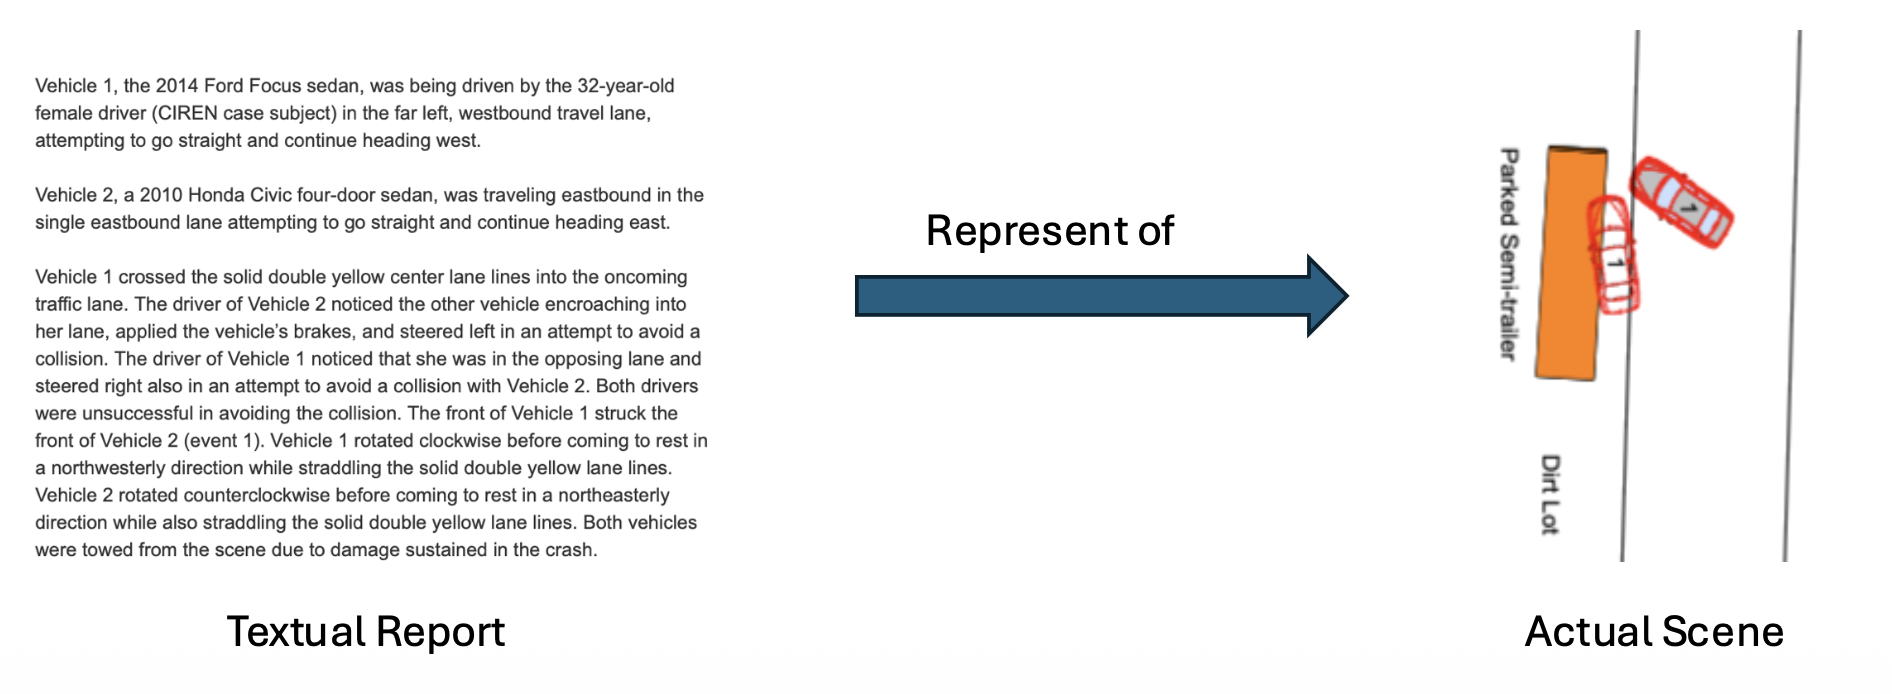
\includegraphics[width=1\textwidth]{images/edge-case-example}
    \caption{ตัวอย่าง Edge Case ที่ซับซ้อนจากรายงานอุบัติเหตุจริง (CIREN) แสดงลำดับเหตุการณ์ที่นำไปสู่การชนประสานงา}
    \label{fig:edge_case_example}
\end{figure}

\subsection{ประสิทธิภาพการค้นพบกรณีขอบเขต (Edge-Case Discovery Efficiency)}
\paragraph{}
การค้นพบ Edge Case ตามที่กล่าวมาข้างต้นมักขาดประสิทธิภาพ กล่าวคือ ต้องสิ้นเปลืองทรัพยากรและเวลาในการสร้างสถานการณ์จำลอง (Scenario) ทั่วไปที่ไม่ท้าทายระบบเป็นจำนวนมาก เพียงเพื่อจะเจอ Edge Case ที่มีความหมายเพียงไม่กี่กรณี แนวคิดเรื่อง ประสิทธิภาพการค้นพบกรณีขอบเขต (Edge-Case Discovery Efficiency) จึงเกิดขึ้นเพื่อวัดผลความสามารถของกระบวนการทดสอบ โดยนิยามว่าคือ อัตราส่วนระหว่างจำนวน Edge Case ที่ค้นพบ ต่อจำนวนสถานการณ์จำลองทั้งหมดที่ถูกสร้างขึ้น

\paragraph{}
งานวิจัยที่เกี่ยวข้องอย่าง \textit{LLMScenario} ได้แสดงให้เห็นถึงความท้าทายนี้ โดยชี้ว่าชุดข้อมูลการขับขี่จริงส่วนใหญ่มักประกอบด้วยสถานการณ์การขับขี่ปกติและปลอดภัย (Normal Safe Scenarios) แต่สถานการณ์ที่มีความเสี่ยงสูง (Extreme Risky Scenarios) ซึ่งถือเป็น Edge Case นั้นมีจำนวนน้อยมาก \cite{chang2023llmscenario} เป้าหมายหลักของงานวิจัยนี้จึงเป็นการเพิ่มประสิทธิภาพดังกล่าวให้สูงที่สุด โดยใช้ Knowledge Graph และ Operational Design Domain (ODD) เป็นกลไกสำคัญในการกรองและมุ่งเป้าการสร้างสถานการณ์จำลองไปยังขอบเขตที่ท้าทายระบบโดยตรง เพื่อลดการสร้าง Scenario ที่ไม่จำเป็นและเร่งการค้นพบ Edge Case ใหม่ให้รวดเร็วยิ่งขึ้น
\section{งานวิจัยที่เกี่ยวข้อง}

\subsection{การสร้างสถานการณ์จำลองจากรายงานอุบัติเหตุ}
\paragraph{}
มีงานวิจัยหลายฉบับที่ได้สำรวจการใช้โมเดลภาษาขนาดใหญ่ (LLM) เพื่อแปลงรายงานอุบัติเหตุเป็นสถานการณ์จำลองสำหรับทดสอบระบบขับขี่อัตโนมัติ (ADS) \cite{khot2024prompting} อย่างไรก็ตาม วิธีการเหล่านี้มักประสบปัญหาสำคัญสองประการคือ ความไม่น่าเชื่อถือของสถานการณ์จำลองที่สร้างขึ้น และการขาดกลไกที่ชัดเจนในการมุ่งเป้าไปยังกรณีขอบเขต (Edge-Case) ที่เกี่ยวข้องกับขอบเขตการทำงานของ ADS โดยตรง ซึ่งงานวิจัยฉบับนี้มุ่งเน้นการแก้ไขปัญหาดังกล่าว

\subsection{การวิเคราะห์อุบัติเหตุด้วย Knowledge Graph}{\label{sec:related_kg_analysis}}
\paragraph{}

\begin{figure}[htbp]
    \centering
    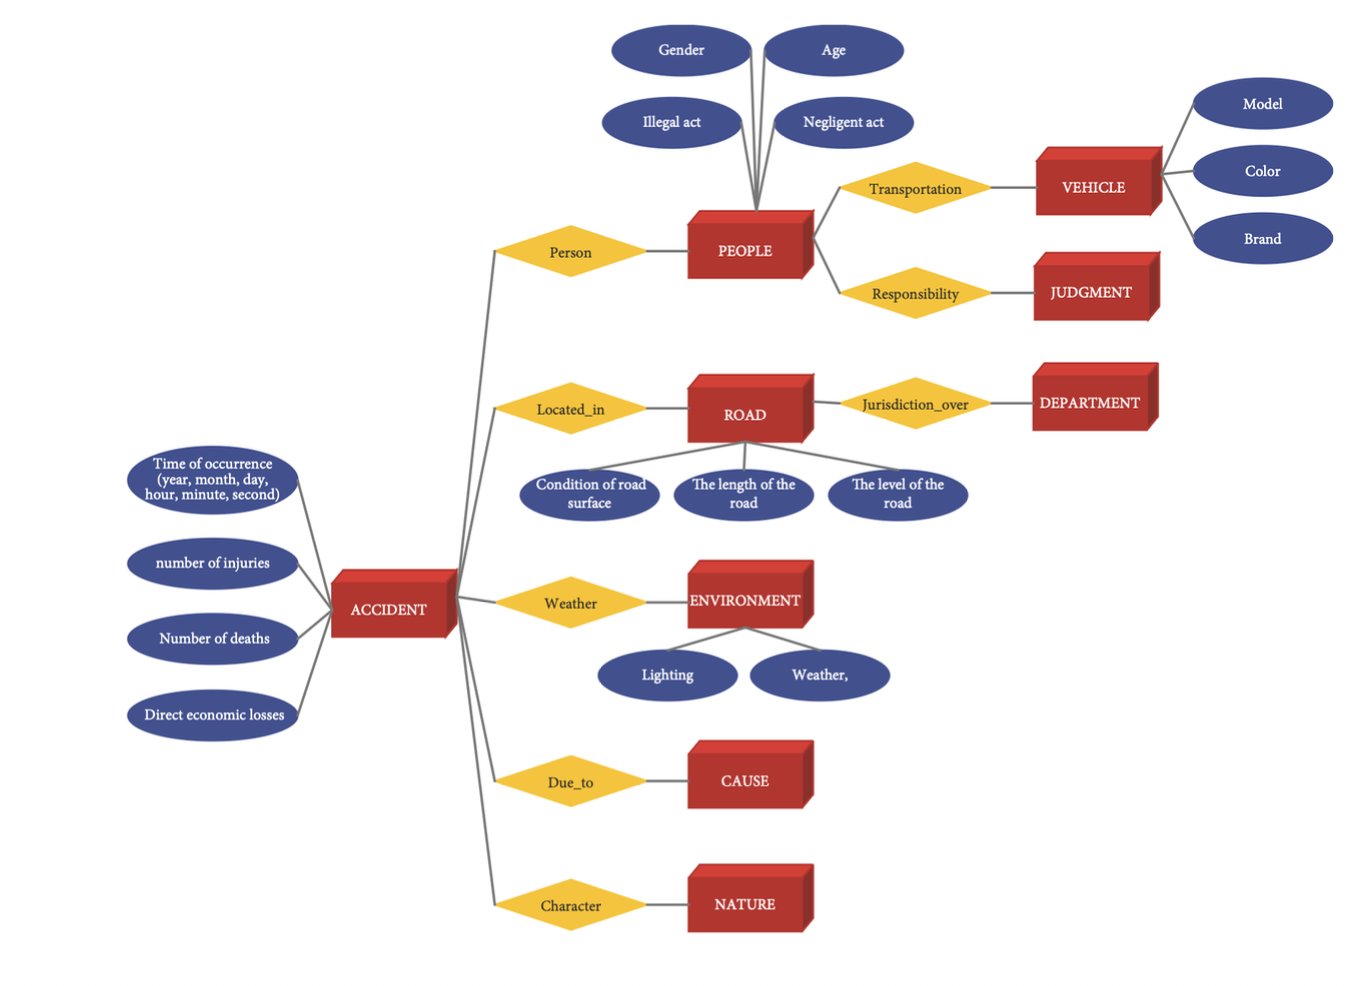
\includegraphics[width=0.9\textwidth]{images/kg-analysis-example}
    \caption{ตัวอย่าง Ontology ของ Knowledge Graph ที่ใช้ในการจำลองความสัมพันธ์ของปัจจัยต่างๆ ในอุบัติเหตุจราจร (ดัดแปลงจาก \cite{liyan2022analysis})}
    \label{fig:kg_analysis_example}
\end{figure}

มีการประยุกต์ใช้ Knowledge Graph (KG) ในการวิเคราะห์อุบัติเหตุจราจร เพื่อจัดระเบียบและแสดงความสัมพันธ์เชิงสาเหตุของปัจจัยต่างๆ ที่นำไปสู่อุบัติเหตุ แนวทางนี้ช่วยให้นักวิจัยสามารถทำความเข้าใจองค์ประกอบที่ซับซ้อนของอุบัติเหตุได้อย่างเป็นระบบ โดยมองแต่ละปัจจัยเป็นเอนทิตี (Entity) ที่เชื่อมโยงกันด้วยความสัมพันธ์ (Relationship) ดังแสดงในรูปที่~\ref{fig:kg_analysis_example} ซึ่งเป็นตัวอย่าง Ontology สำหรับอุบัติเหตุจากงานวิจัยของ Zhang และคณะ~\cite{liyan2022analysis}


\paragraph{}
จากภาพจะเห็นว่า KG สามารถเชื่อมโยงข้อมูลจากหลากหลายมิติเข้าด้วยกัน เช่น \textbf{ACCIDENT} (อุบัติเหตุ) เกิดขึ้นกับ \textbf{PEOPLE} (บุคคล) และ \textbf{VEHICLE} (ยานพาหนะ) ในสภาพ \textbf{ENVIRONMENT} (สิ่งแวดล้อม) และ \textbf{ROAD} (ถนน) ที่เฉพาะเจาะจง ซึ่งการใช้โครงสร้าง KG นี้ช่วยในการอนุมานข้อมูลที่อาจขาดหายไปและเพิ่มความเข้าใจในภาพรวมของเหตุการณ์ได้เป็นอย่างดี อย่างไรก็ตาม งานวิจัยในกลุ่มนี้มักมุ่งเน้นที่การ วิเคราะห์เพื่อความเข้าใจ มากกว่าการนำไปประยุกต์ใช้เพื่อ สร้างชุดทดสอบที่มีเป้าหมายเฉพาะ ซึ่งเป็นช่องว่างที่งานวิจัยฉบับนี้ต้องการจะเติมเต็ม

\subsection{การประยุกต์ใช้ ODD ในการทดสอบ}

\begin{figure}[htbp]
    \centering
    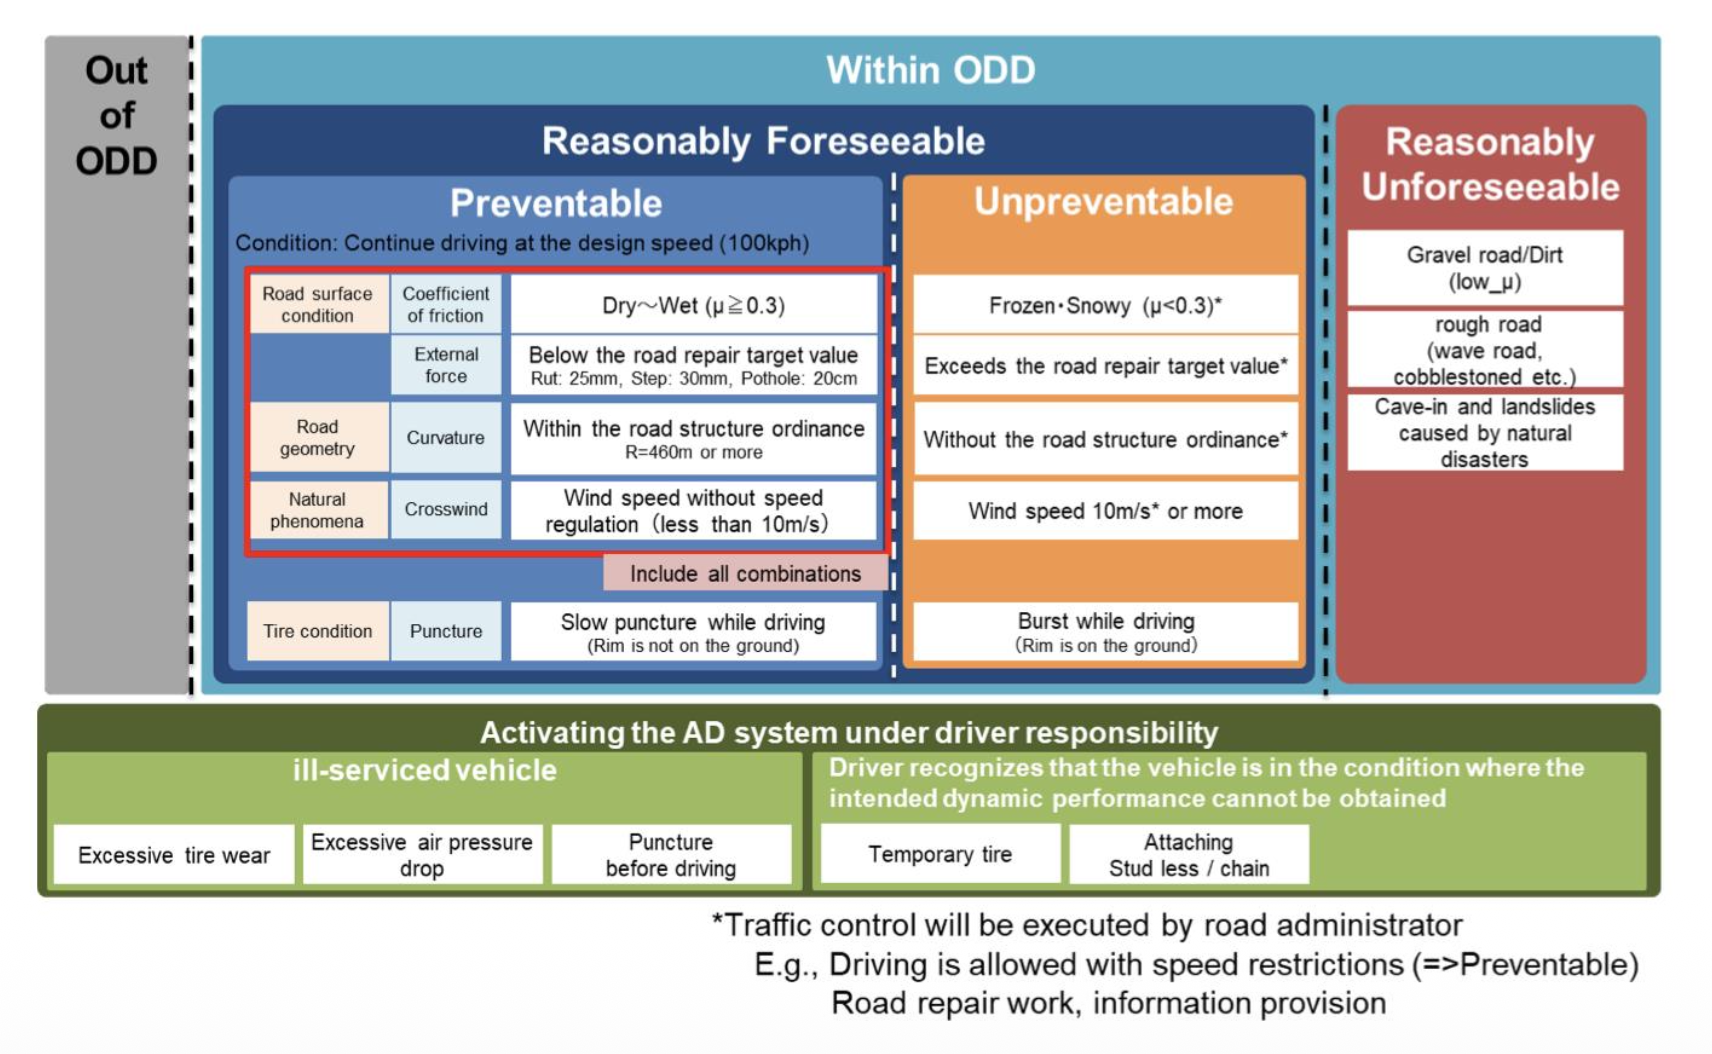
\includegraphics[width=1\textwidth]{images/jama-odd-example}
    \caption{ตัวอย่างการจำแนกสถานการณ์ตามกรอบการทำงาน ODD ของ JAMA \cite{jama2022framework}}
    \label{fig:jama_odd_example}
\end{figure}

\paragraph{}
มีงานวิจัยและกรอบการทำงานในอุตสาหกรรมหลายฉบับที่ได้เสนอแนวคิดในการใช้ออนโทโลยี (Ontology) หรือ Operational Design Domain (ODD) เพื่อจัดหมวดหมู่และกำหนดขอบเขตของการสร้างสถานการณ์จำลองสำหรับยานยนต์อัตโนมัติ \cite{bagschik2018ontology} แนวทางนี้ช่วยให้การทดสอบมีเป้าหมายที่ชัดเจนและเป็นระบบมากขึ้น โดยหนึ่งในกรอบการทำงานที่เป็นที่ยอมรับอย่างกว้างขวางคือ \textbf{Automated Driving Safety Evaluation Framework} โดย \textbf{JAMA} \cite{jama2022framework}

\paragraph{}
กรอบการทำงานของ JAMA ได้แบ่งประเภทของสถานการณ์การขับขี่ตามเงื่อนไขต่างๆ เช่น สภาพถนน, สภาพอากาศ, และรูปทรงของถนน เพื่อกำหนดขอบเขตการทำงานที่ปลอดภัยของระบบ ADS อย่างชัดเจน ดังแสดงในรูปที่~\ref{fig:jama_odd_example} ซึ่งจำแนกสถานการณ์ออกเป็น 3 ส่วนหลักคือ: \textbf{Preventable} (ป้องกันได้), \textbf{Unpreventable} (ป้องกันไม่ได้) ภายในขอบเขตที่คาดการณ์ได้ (Reasonably Foreseeable), และสถานการณ์ที่อยู่นอกขอบเขต ODD โดยสิ้นเชิง (Out of ODD) การจัดหมวดหมู่นี้ช่วยให้ผู้พัฒนาระบบสามารถออกแบบการทดสอบที่สอดคล้องกับความสามารถของ ADS ได้อย่างแม่นยำ


\paragraph{}
อย่างไรก็ตาม แม้แนวทางเหล่านี้จะช่วยกำหนดขอบเขตการทดสอบได้ดี แต่ยังไม่มีการผสานรวม ODD เข้ากับโครงสร้าง Knowledge Graph และ LLM อย่างเป็นระบบ เพื่อแก้ไขปัญหาประสิทธิภาพในการค้นพบ Edge-Case โดยตรง ซึ่งเป็นช่องว่างสำคัญที่งานวิจัยฉบับนี้มุ่งเน้นที่จะพัฒนา
\subsection{ความแตกต่างและช่องว่างทางการวิจัย}
\paragraph{}
หัวใจสำคัญของปัญหาที่งานวิจัยนี้มุ่งเน้นแก้ไขคือ "ประสิทธิภาพในการค้นพบกรณีขอบเขต" (Edge-Case Discovery Efficiency) ที่ต่ำในวิธีการทั่วไป งานวิจัยก่อนหน้าอย่าง \textit{LLMScenario} ได้แสดงให้เห็นอย่างชัดเจนว่าข้อมูลการขับขี่ในโลกแห่งความเป็นจริงส่วนใหญ่มหาศาลประกอบด้วยสถานการณ์ที่ปลอดภัยและเกิดขึ้นเป็นปกติ (Normal Safe Scenarios) ในขณะที่สถานการณ์ที่มีความเสี่ยงสูง (Extreme Risky Scenarios) ซึ่งเป็น Edge-Case ที่มีความสำคัญต่อการทดสอบนั้นมีอยู่น้อยมาก \cite{chang2023llmscenario} ทำให้การสร้างสถานการณ์จำลองโดยขาดการชี้นำเป้าหมายต้องสร้างเหตุการณ์ซ้ำๆ จำนวนมากจนกว่าจะพบเหตุการณ์ใหม่ที่ท้าทายระบบอย่างแท้จริง ดังแสดงในรูปที่~\ref{fig:llmscenario_distribution}

\begin{figure}[htbp]
    \centering
    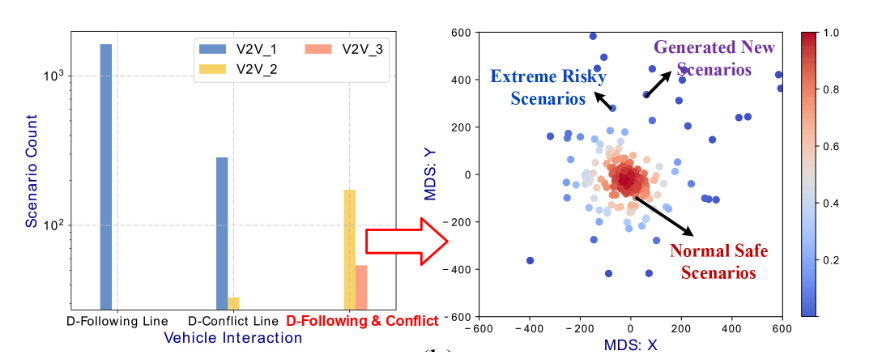
\includegraphics[width=0.9\textwidth]{images/llmscenario-distribution}
    \caption{การกระจายตัวของสถานการณ์ที่แสดงให้เห็นถึงความหนาแน่นของ Normal Safe Scenarios (กลุ่มสีแดงตรงกลาง) เทียบกับ Extreme Risky Scenarios ที่กระจัดกระจาย ซึ่งชี้ให้เห็นถึงความยากในการค้นพบเหตุการณ์หายาก (ดัดแปลงจาก \cite{chang2023llmscenario})}
    \label{fig:llmscenario_distribution}
\end{figure}

\paragraph{}
งานวิจัยฉบับนี้จึงเติมเต็มช่องว่างดังกล่าว โดยนำเสนอแนวทางการแก้ปัญหาแบบบูรณาการเป็นครั้งแรก ซึ่งเป็นการสังเคราะห์จุดแข็งของเทคโนโลยีสามส่วนเข้าไว้ด้วยกัน ได้แก่ 1) ความน่าเชื่อถือของ Knowledge Graph, 2) ความสามารถของ Schema-guided LLM, และ 3) การกำหนดขอบเขตที่ชัดเจนของ Operational Design Domain (ODD) การผสานรวมเทคโนโลยีทั้งสามส่วนนี้เข้าไว้ในกรอบการทำงานเดียว (ดังแสดงในรูปที่~\ref{fig:system_architecture_overview}) ทำให้เกิดเป็นแนวทางใหม่ที่มุ่งเน้นการแก้ไขปัญหา Edge-Case Discovery Efficiency โดยเฉพาะ ซึ่งแตกต่างจากงานวิจัยก่อนหน้าที่มักจะมุ่งเน้นเพียงเทคโนโลยีใดเทคโนโลยีหนึ่งเท่านั้น

\begin{figure}[htbp]
    \centering
    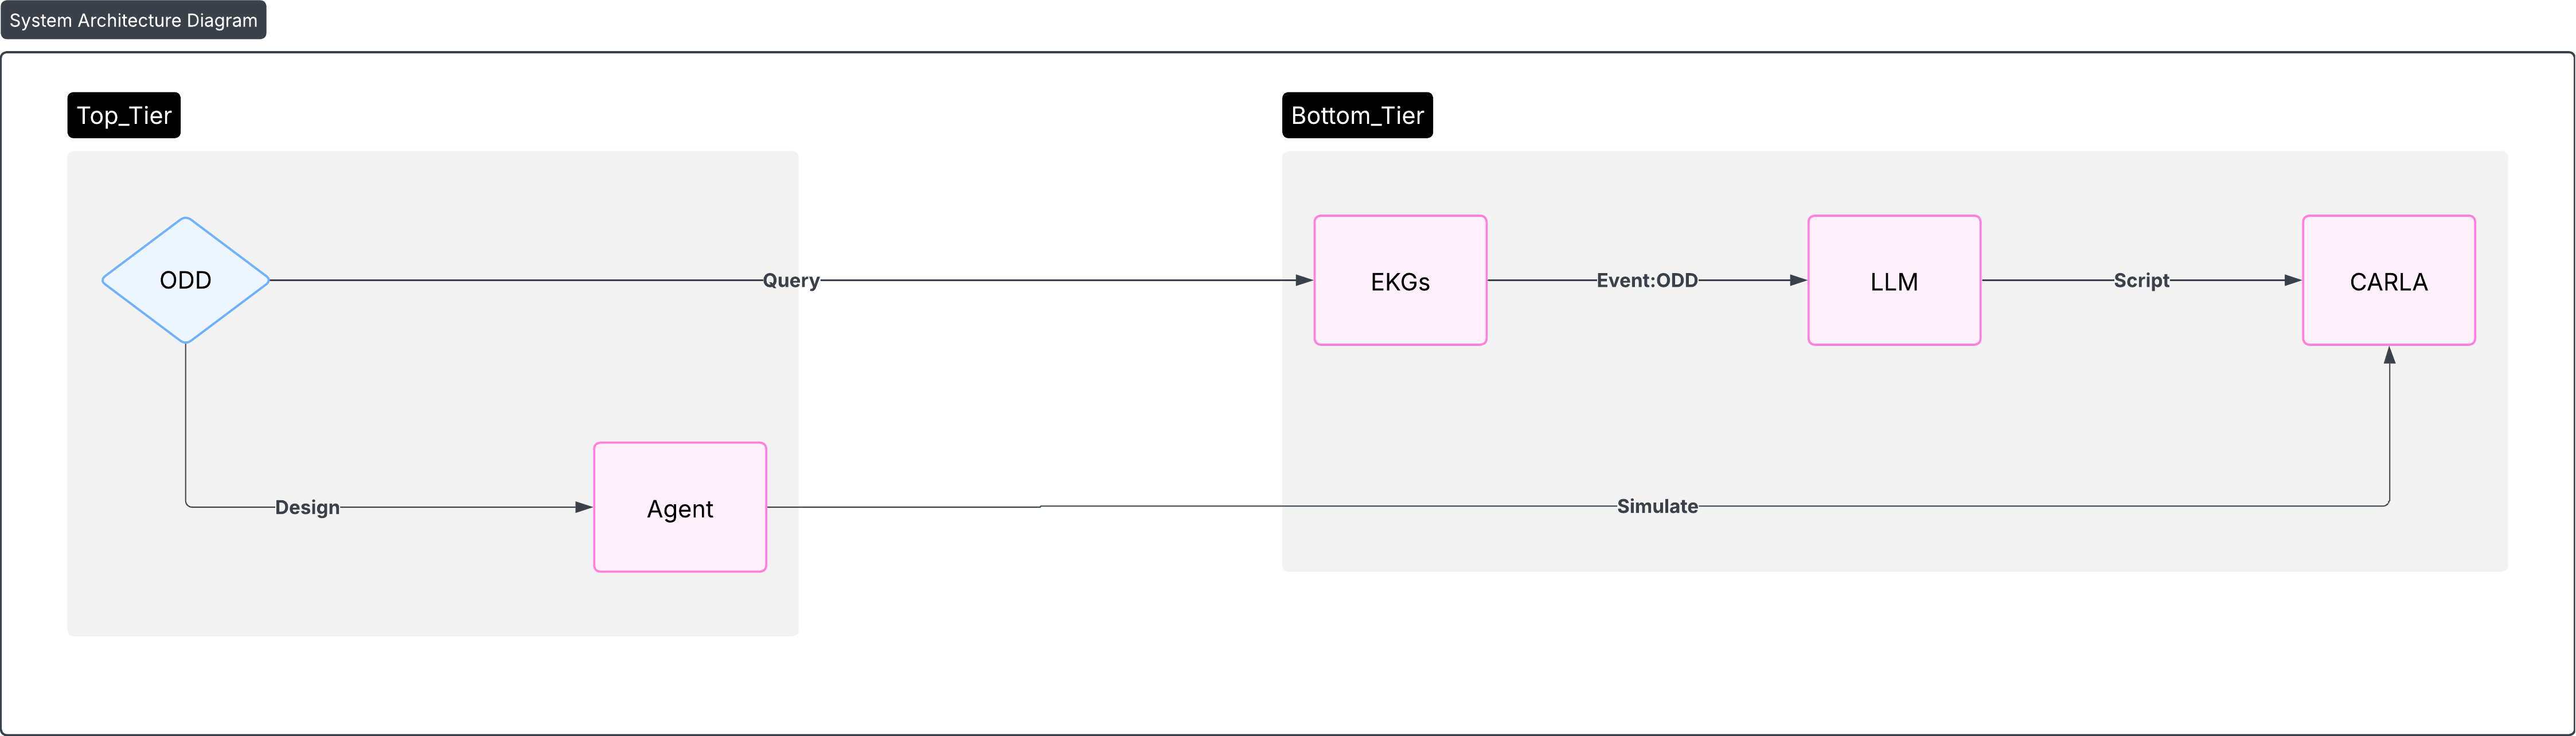
\includegraphics[width=0.8\textwidth]{images/system-architecture-overview}
    \caption{แผนภาพสถาปัตยกรรมภาพรวมของกรอบการทำงาน ที่แสดงการบูรณาการ ODD, Knowledge Graph, และ LLM เข้าด้วยกันเพื่อสร้างชุดทดสอบ}
    \label{fig:system_architecture_overview}
\end{figure}

\section{เทคโนโลยีและเครื่องมือที่ใช้}

\subsection{เครื่องมือประมวลผลภาษาธรรมชาติและข้อมูล}
\begin{itemize}
    \item \textbf{Large Language Model (LLM):} งานวิจัยนี้เลือกใช้โมเดล \textbf{GPT-4o} \cite{openai2024gpt4o} เป็นเครื่องมือหลักในการทำ Schema-guided Extraction เหตุผลสำคัญที่เลือกใช้โมเดลนี้คือความสามารถแบบหลายรูปแบบ (Multimodality) โดยเฉพาะความสามารถในการประมวลผลภาพ (Vision) ซึ่งทำให้ GPT-4o สามารถวิเคราะห์ รายงานที่เป็นข้อความ (Textual Narrative) ได้พร้อมกัน ความสามารถนี้ช่วยเพิ่มความแม่นยำในการสกัดข้อมูลที่มีความสัมพันธ์เชิงพื้นที่ (Spatial Relationship) เช่น ทิศทางการเคลื่อนที่ของรถยนต์ และตำแหน่งที่เกิดการชน ซึ่งเป็นข้อมูลที่อาจกำกวมหากอ่านจากข้อความเพียงอย่างเดียว

    \item \textbf{Knowledge Graph Database:} ใช้แพลตฟอร์มฐานข้อมูลเชิงกราฟ เช่น Neo4j \cite{neo4j} ซึ่งเหมาะสมกับการจัดเก็บข้อมูลที่มีความสัมพันธ์ซับซ้อนอย่าง KG และรองรับการทำ Inference Engine เพื่อตรวจสอบข้อจำกัดของ ODD
\end{itemize}

\subsection{แหล่งข้อมูลอุบัติเหตุ}\label{subsec:accident-data-sources}
\paragraph{}
งานวิจัยนี้อาศัยข้อมูลจากฐานข้อมูลอุบัติเหตุจริงเชิงลึกที่เปิดเผยต่อสาธารณะ เพื่อใช้เป็นข้อมูลนำเข้าในการสกัดสถานการณ์จำลอง แหล่งข้อมูลหลักประกอบด้วยฐานข้อมูลสำคัญสองแห่งคือ CIREN และ GIDAS ซึ่งมีลักษณะและตัวอย่างข้อมูลดังต่อไปนี้

\subsubsection{CIREN (Crash Injury Research and Engineering Network)}
\paragraph{}
CIREN เป็นเครือข่ายวิจัยการบาดเจ็บจากอุบัติเหตุของหน่วยงาน NHTSA ในสหรัฐอเมริกา \cite{nhtsa_ciren} จุดเด่นของ CIREN คือรายงานที่มีความละเอียดสูงมาก ประกอบด้วยคำบรรยายลำดับเหตุการณ์ (Narrative) ข้อมูลเชิงวิศวกรรม และข้อมูลทางการแพทย์อย่างครบถ้วน ดังตัวอย่างกรณีศึกษาในรูปที่~\ref{fig:ciren_example}

\begin{figure}[h!]
    \centering
    \begin{minipage}{0.48\textwidth}
        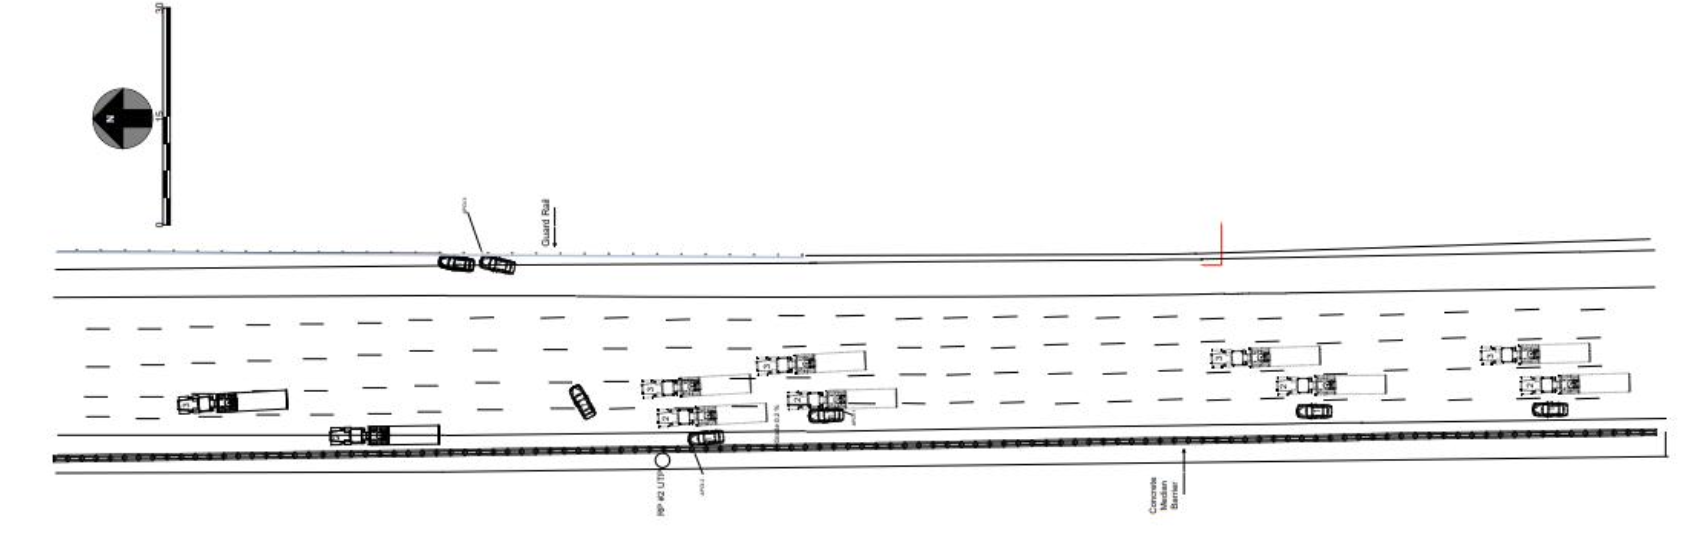
\includegraphics[width=\linewidth]{images/ciren-case-example}
    \end{minipage}\hfill
    \begin{minipage}{0.48\textwidth}
        \footnotesize
        \textenglish{V1 was traveling northbound in lane five of a five lane controlled access roadway. V2 was traveling in lane four next to V1. A non-contact Medium-Heavy truck was traveling next to V2 in lane three when it began to change lanes to the left forcing V2 to also change lanes to the left. When changing lanes to the left the left side of V2's trailer contacted the right side of V1. This contact forced V1 to depart the roadway where the left side of V1 contacted a concrete barrier before continuing to travel forward across all five lanes to depart the roadway on the right, where the front of V1 contacted the guardrail face before coming to final rest.}
    \end{minipage}
    \caption{ตัวอย่างกรณีศึกษาและคำอธิบายเหตุการณ์จากฐานข้อมูล CIREN (Case \#1-10-2017-003-09)}
    \label{fig:ciren_example}
\end{figure}

\subsubsection{GIDAS (German In-Depth Accident Study)}
\paragraph{}
GIDAS เป็นโครงการรวบรวมข้อมูลอุบัติเหตุเชิงลึกในประเทศเยอรมนี \cite{gidas_study} ซึ่งมีขนาดใหญ่และครอบคลุมความรุนแรงของอุบัติเหตุที่หลากหลาย ตั้งแต่กรณีเล็กน้อยไปจนถึงรุนแรง ทำให้เหมาะสำหรับการวิเคราะห์เชิงสถิติเพื่อทำความเข้าใจการกระจายตัวของข้อมูลอุบัติเหตุจริง ดังตัวอย่างกรณีศึกษาในรูปที่~\ref{fig:gidas_example}

\begin{figure}[h!]
    \centering
    \begin{minipage}{0.48\textwidth}
        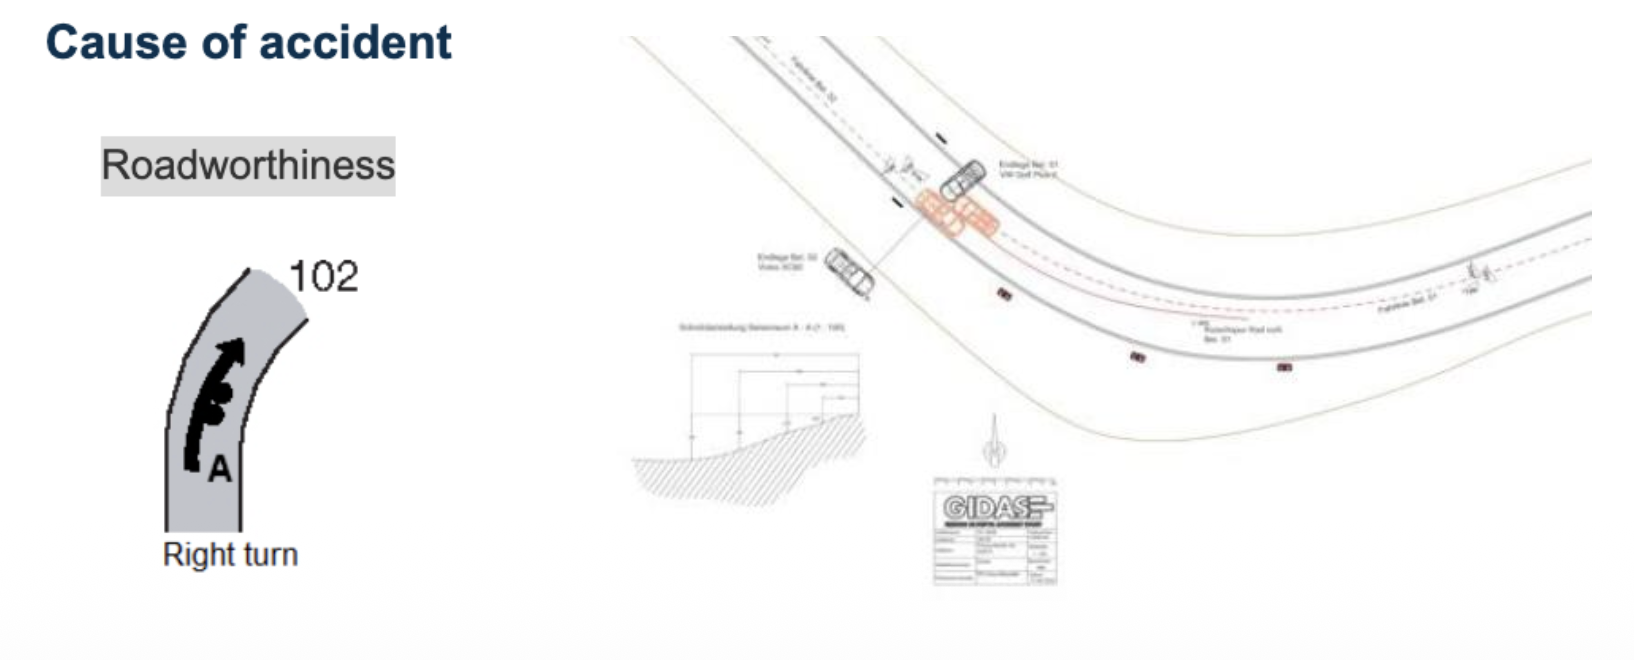
\includegraphics[width=\linewidth]{images/gidas-case-example}
    \end{minipage}\hfill
    \begin{minipage}{0.48\textwidth}
        \footnotesize
        \textenglish{Participant 01 (VW Golf) was driving on the K9013 in the direction of Oelsa. He skidded on a downhill section in a right-hand bend on a wet road surface. The vehicle understeers and collides with participant 02 (Volvo XC60), who is driving on the K9013 in the opposite direction. As a result of the collision, the car 02 slides into the embankment. Both occupants of participant 01 and the driver of participant 02 are slightly injured.}
    \end{minipage}
    \caption{ตัวอย่างกรณีศึกษาและคำอธิบายเหตุการณ์จากฐานข้อมูล GIDAS}
    \label{fig:gidas_example}
\end{figure}

\paragraph{}
ข้อมูลจากแหล่งข้อมูลทั้งสองดังที่แสดงในตัวอย่าง มีความละเอียดเพียงพอต่อการสกัดเอนทิตีและความสัมพันธ์เพื่อสร้างเป็น Knowledge Graph ได้อย่างสมบูรณ์

\subsection{มาตรฐานและสภาพแวดล้อมจำลอง}\label{subsec:ch2_standards}
\paragraph{}
ผลลัพธ์สุดท้ายของกรอบการทำงานวิจัยนี้ ถูกออกแบบให้สามารถส่งออกสถานการณ์จำลอง (Scenario) ในรูปแบบไฟล์ที่เข้ากันได้กับมาตรฐานอุตสาหกรรมยานยนต์ นั่นคือ \textbf{ASAM OpenSCENARIO} ซึ่งเป็นรูปแบบมาตรฐานที่ใช้ในการอธิบายลำดับเหตุการณ์ พฤติกรรมของ Actors, และเงื่อนไขต่างๆ ในการทดสอบระบบขับขี่อัตโนมัติ การใช้มาตรฐานนี้ช่วยให้ชุดทดสอบที่สร้างขึ้นสามารถนำไปใช้งานในสภาพแวดล้อมจำลอง (Simulation Environment) ที่หลากหลายได้ เช่น CARLA, Esmini, VTD เป็นต้น

\paragraph{}
เพื่อแสดงให้เห็นภาพผลลัพธ์ที่เป็นรูปธรรม ขอนำเสนอตัวอย่างโค้ดของไฟล์ OpenSCENARIO (`.xosc`) ซึ่งเป็นไฟล์ XML ที่อธิบายสถานการณ์จำลอง "รถยนต์ขับตัดหน้า (Cut-in)" ฉบับย่อ ดังแสดงในโค้ดตัวอย่างที่~\ref{lst:openscenario_example}

\newpage % --- คำสั่งขึ้นหน้าใหม่ ---

\begin{lstlisting}[language=XML, caption={ตัวอย่างโค้ดไฟล์ ASAM OpenSCENARIO ฉบับย่อ ที่อธิบายสถานการณ์ Cut-in}, label={lst:openscenario_example}]
<OpenSCENARIO>
  <Entities>
    <ScenarioObject name="Ego">
      <Vehicle name="DefaultVehicle" vehicleCategory="car"/>
    </ScenarioObject>
    <ScenarioObject name="Adversary">
      <Vehicle name="DefaultVehicle" vehicleCategory="car"/>
    </ScenarioObject>
  </Entities>

  <Storyboard>
    <Init>
      <Actions>
        <Private entityRef="Ego">
           </Private>
        <Private entityRef="Adversary">
           </Private>
      </Actions>
    </Init>
    <Story name="CutInStory">
      <Act name="CutInAct">
        <ManeuverGroup name="AdversaryManeuver">
          <Actors>
            <EntityRef entityRef="Adversary"/>
          </Actors>
          <Maneuver name="AdversaryCutIn">
            <Event name="AdversaryLaneChange" priority="parallel">
              <Action name="LaneChangeAction">
                <PrivateAction>
                  <LaneChangeAction>
                    <LaneChangeTarget>
                      <RelativeTargetLane entityRef="Ego" value="0"/>
                    </LaneChangeTarget>
                  </LaneChangeAction>
                </PrivateAction>
              </Action>
              <StartTrigger>
                </StartTrigger>
            </Event>
          </Maneuver>
        </ManeuverGroup>
        <StartTrigger/>
      </Act>
    </Story>
  </Storyboard>
</OpenSCENARIO>
\end{lstlisting}

\paragraph{}
จากโค้ดตัวอย่างจะเห็นองค์ประกอบสำคัญต่างๆ เช่น ส่วน `<Entities>` ใช้สำหรับประกาศ Actors ที่เกี่ยวข้อง (รถ Ego และรถคู่กรณี), ส่วน `<Init>` ใช้วางตำแหน่งเริ่มต้นของรถแต่ละคัน และส่วน `<Storyboard>` ซึ่งเป็นหัวใจหลัก ใช้อธิบายลำดับเหตุการณ์และพฤติกรรมที่จะเกิดขึ้น เช่น การเปลี่ยนเลนเพื่อขับตัดหน้า (`<LaneChangeAction>`) กรอบการทำงานวิจัยนี้จะทำหน้าที่สร้างไฟล์ที่มีโครงสร้างลักษณะนี้ขึ้นมาโดยอัตโนมัติจากข้อมูลอุบัติเหตุจริง